\section*{Results}

Our first successful keep-alive connection, where you can see that one thread is reused for multiple requests. %TODO: why not for all requests the same thread ?  
And a simple CGI Script where we display the environment variables REMOTE\_HOST and REMOTE\_ADDR. 

\begin{figure}[h]
    \centering
    \begin{minipage}{0.55\textwidth}
        \centering
        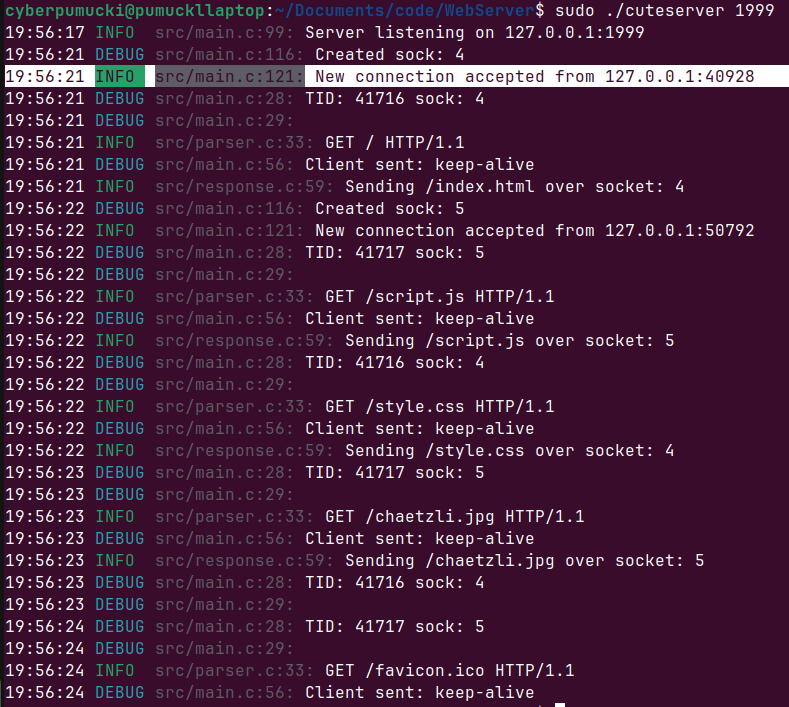
\includegraphics[width=\textwidth]{figures/keep-alive.png}
        \caption{Keep-Alive: Multiple Requests handled over one Connection}
    \end{minipage}
    \hfill
    \begin{minipage}{0.35\textwidth}
        \centering
        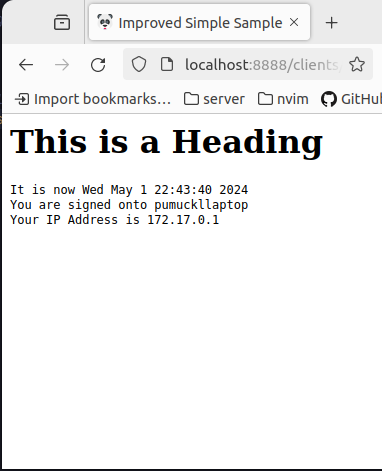
\includegraphics[width=\textwidth]{figures/cgi.png}
        \caption{First simple CGI Script with Env Variables}
    \end{minipage}
\end{figure}

\subsection*{Performance Testing}
We wanted to test the influence of the number of worker threads on the performance of our application. For this we used \textbf{Locust} \footnote{https://locust.io/} to get and post messages from/to the application on the server. Locust Configuration: 100 users, ramp up 10 users/second, running for 60 seconds. We then ran the application multiple times, with a different number of workers defined in our config.toml. 
% TODO:Locust Plot, discuss results

\begin{figure}[h]
    \centering
    \begin{minipage}{0.45\textwidth}
        \centering
        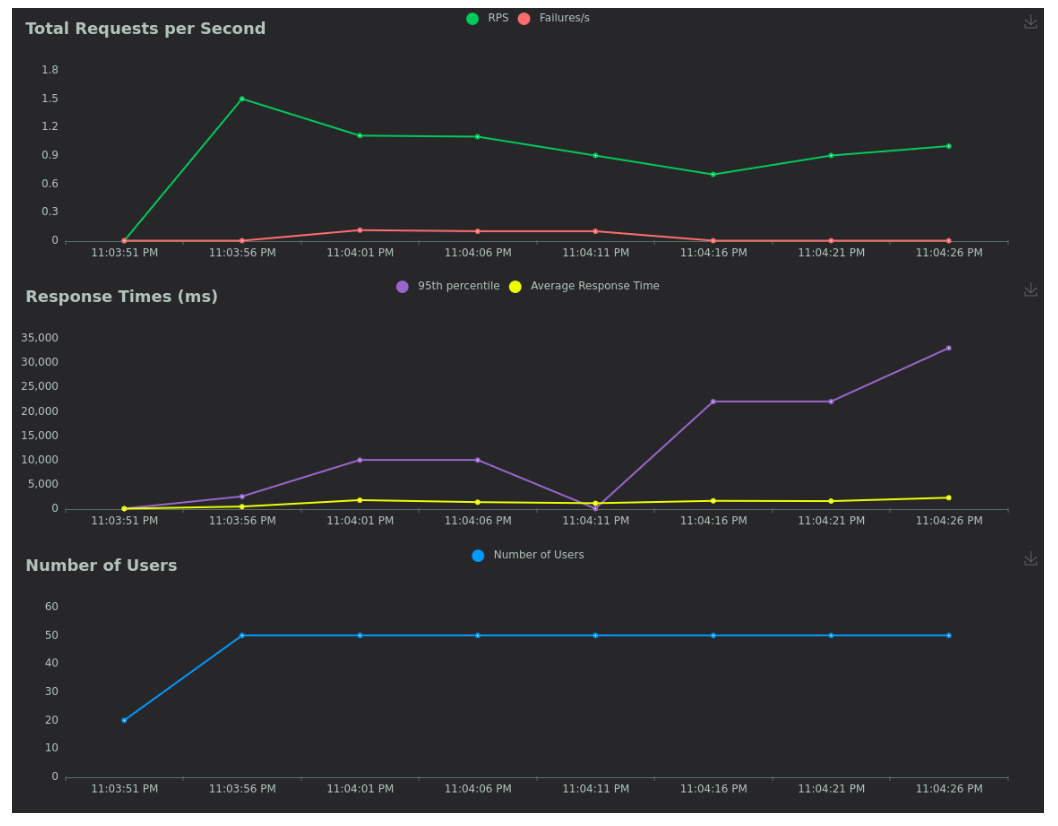
\includegraphics[width=\textwidth]{figures/report_2_threads.png}
        \caption{Results with 2 Worker Threads}
    \end{minipage}
    \hfill
    \begin{minipage}{0.45\textwidth}
        \centering
        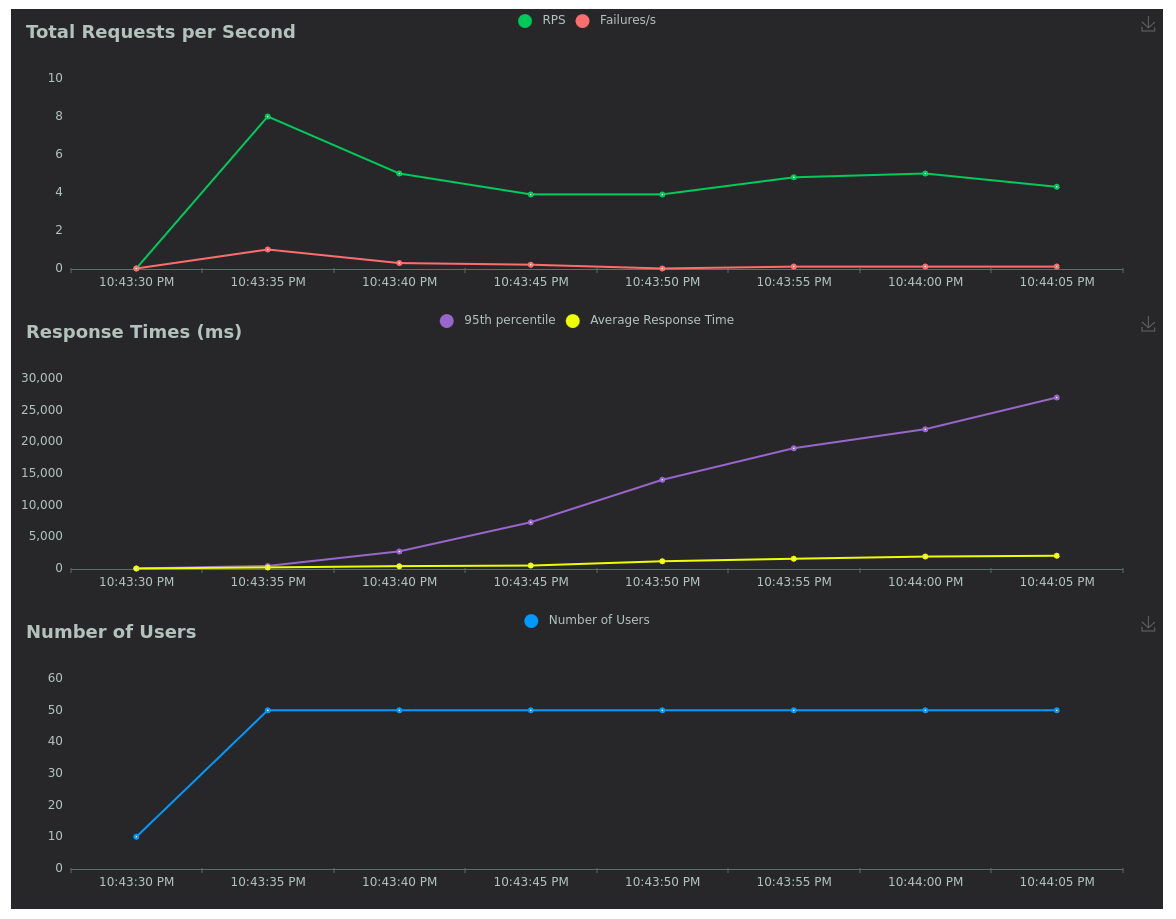
\includegraphics[width=\textwidth]{figures/report_10_threads.png}
        \caption{Results with 10 Worker Threads}
    \end{minipage}
\end{figure}


